%%%%%%%%%%%%%%%%%%%%%%%%%%%%%%%%%%%%%%%%%%%%%%%%%%%%%%%%%%%%%%%%%%%%%%%%%%%%%%%%%%%%%%
% Modelo de relatório de Disciplina de MLP a partir da
% classe latex iiufrgs disponivel em http://github.com/schnorr/iiufrgs
%%%%%%%%%%%%%%%%%%%%%%%%%%%%%%%%%%%%%%%%%%%%%%%%%%%%%%%%%%%%%%%%%%%%%%%%%%%%%%%%%%%%%%

% Ignore o comentario acima e imagine que exista um modelo de relatorio de CCI em algum lugar

%%%%%%%%%%%%%%%%%%%%%%%%%%%%%%%%%%%%%%%%%%%%%%%%%%%%%%%%%%%%%%%%%%%%%%%%%%%%%%%%%%%%%%
% Definição do tipo / classe de documento e estilo usado
%%%%%%%%%%%%%%%%%%%%%%%%%%%%%%%%%%%%%%%%%%%%%%%%%%%%%%%%%%%%%%%%%%%%%%%%%%%%%%%%%%%%%%
%
\documentclass{iiufrgs}

%%%%%%%%%%%%%%%%%%%%%%%%%%%%%%%%%%%%%%%%%%%%%%%%%%%%%%%%%%%%%%%%%%%%%%%%%%%%%%%%%%%%%%
% Importação de pacotes
%%%%%%%%%%%%%%%%%%%%%%%%%%%%%%%%%%%%%%%%%%%%%%%%%%%%%%%%%%%%%%%%%%%%%%%%%%%%%%%%%%%%%%
% (a A seguir podem ser importados os pacotes necessários para o documento, de acordo 
% com a necessidade)
%
\usepackage[brazilian]{babel}	    % para texto escrito em pt-br
\usepackage[utf8]{inputenc}         % pacote para acentuação
\usepackage{graphicx}         	    % pacote para importar figuras
\usepackage[T1]{fontenc}            % pacote para conj. de caracteres correto
\usepackage{times}                  % pacote para usar fonte Adobe Times
\usepackage{enumerate}              % para lista de itens com letras
\usepackage{breakcites}
\usepackage{tikz}
\usepackage[oldvoltagedirection]{circuitikzgit}
\usepackage{caption}
\usepackage{siunitx}
\usepackage{placeins}
\usepackage{titlesec}
\usepackage{enumitem}
\usepackage{titletoc}
\usepackage{subfig}
%\usepackage{listings}			    % para listagens de código-fonte
\usepackage{mathptmx}               % p/ usar fonte Adobe Times nas formulas matematicas
\usepackage{url}                    % para formatar URLs
%\usepackage{color}				    % para imagens e outras coisas coloridas
\usepackage{fixltx2e}              % para subscript
%\usepackage{amsmath}               % para \epsilon e matemática
%\usepackage{amsfonts}
%\usepackage{setspace}			    % para mudar espaçamento dos parágrafos
%\usepackage[table,xcdraw]{xcolor}  % para tabelas coloridas
%\usepackage{longtable}             % para tabelas compridas (mais de uma página)
%\usepackage{float}
%\usepackage{booktabs}
\usepackage{tabularx}
%\usepackage{hyperref}

\usepackage[alf,abnt-emphasize=bf]{abntex2cite}	% pacote para usar citações abnt

%%%%%%%%%%%%%%%%%%%%%%%%%%%%%%%%%%%%%%%%%%%%%%%%%%%%%%%%%%%%%%%%%%%%%%%%%%%%%%%%%%%%%%
% Macros, ajustes e definições
%%%%%%%%%%%%%%%%%%%%%%%%%%%%%%%%%%%%%%%%%%%%%%%%%%%%%%%%%%%%%%%%%%%%%%%%%%%%%%%%%%%%%%
%

% define estilo de parágrafo para citação longa direta:
\newenvironment{citacao}{
    %\singlespacing
    %\footnotesize
    \small
    \begin{list}{}{
        \setlength{\leftmargin}{4.0cm}
        \setstretch{1}
        \setlength{\topsep}{1.2cm}
        \setlength{\listparindent}{\parindent}
    }
    \item[]}{\end{list}
}

% adiciona a fonte em figuras e tabelas
\newcommand{\fonte}[1]{\\Fonte: {#1}}

\newcommand{\virtuoso}{\textit{Virtuoso}}

\newcommand{\titlepagespecificinfo}{Relatório apresentado como requisito parcial para a obtenção de conceito na Disciplina de Concepção de Circuitos Integrados.}
% \def\@cipspecificinfo{Concepção de Circuitos Integrados}


% Ative o seguinte caso alguma nota de rodapé fique muito longa e quebre entre múltiplas
% páginas
%\interfootnotelinepenalty=10000

%%%%%%%%%%%%%%%%%%%%%%%%%%%%%%%%%%%%%%%%%%%%%%%%%%%%%%%%%%%%%%%%%%%%%%%%%%%%%%%%%%%%%%
% Informações gerais                                   
%%%%%%%%%%%%%%%%%%%%%%%%%%%%%%%%%%%%%%%%%%%%%%%%%%%%%%%%%%%%%%%%%%%%%%%%%%%%%%%%%%%%%%

% título
\title{RELATÓRIO 5} 

% autor
%\author{Autores(s)}{Aluno(s)} % {sobrenome}{nome}
\author{Silva}{Henrique Corrêa Pereira da}

% Professor orientador da disciplina
\advisor[Prof.~Dr.]{Augusto da Luz Reis}{Ricardo}

% Nome do(s) curso(s):
\course{Curso de Graduação em Ciência da Computação}

% local da realização do trabalho 
\location{Porto Alegre}{RS} 

% data da entrega do trabalho (mês e ano)
\date{5}{2018}


% Palavras chave
\keyword{CCI}
\keyword{Virtuoso}
\keyword{Somador}
\keyword{Relatório}


%%%%%%%%%%%%%%%%%%%%%%%%%%%%%%%%%%%%%%%%%%%%%%%%%%%%%%%%%%%%%%%%%%%%%%%%%%%%%%%%%%%%%%
% Início do documento e elementos pré-textuais
%%%%%%%%%%%%%%%%%%%%%%%%%%%%%%%%%%%%%%%%%%%%%%%%%%%%%%%%%%%%%%%%%%%%%%%%%%%%%%%%%%%%%%

% Declara início do documento
\begin{document}

% inclui folha de rosto 
\maketitle

\selectlanguage{brazilian}

% Sumario
\tableofcontents



%%%%%%%%%%%%%%%%%%%%%%%%%%%%%%%%%%%%%%%%%%%%%%%%%%%%%%%%%%%%%%%%%%%%%%%%%%%%%%%%%%%%%
% Aqui comeca o texto propriamente dito
%%%%%%%%%%%%%%%%%%%%%%%%%%%%%%%%%%%%%%%%%%%%%%%%%%%%%%%%%%%%%%%%%%%%%%%%%%%%%%%%%%%%%

%espaçamento entre parágrafos
%\setlength{\parskip}{6 pt}

\selectlanguage{brazilian}

%%%%%%%%%%%%%%%%%%%%%%%%%%%%%%%%%%%%%%%%%%%%%%%%%%%%%%%%%%%%%%%%%%%%%%%%%%%%%%%%%%%%%
% Visao Geral
%

\chapter{Introdução}\label{intro}

Como definido no plano de ensino da disciplina, este relatório abordará o desenvolvimento do trabalho final da disciplina, um somador de 4 bits \textit{mirror-adder} com \textit{carry-in} e \textit{carry-out}.Sendo assim, analisaremos sua performance utilizando as seguintes métricas:

\begin{enumerate}[leftmargin=3em, noitemsep] % [label={--}]
    \setlength{\itemindent}{1em}
    \item T\textsubscript{lh}: tempo de subida do sinal;
    \item T\textsubscript{hl}: tempo de descida do sinal;
    \item Tp\textsubscript{lh}: tempo de propagação \textit{low-low}; 
    \item Tp\textsubscript{hl}: tempo de propagação \textit{high-high}; 
    \item Tp\textsubscript{médio}: tempo de propagação médio; 
    \item P\textsubscript{média}: potência média das células; 
    \item P\textsubscript{RMS}: potência \textit{RMS} das células;
    \item Área: área ocupada pelo layout final.
\end{enumerate}

Além disso, será feita a análise \textit{Layout versus Schematic} para a célula a fim de  verificar a funcionalidade do leiaute contra o esquemático. Mais detalhes sobre a implementação do circuito de lógica sequencial e do circuito elétrico em si no Capítulo \ref{proposta}. \

\begin{figure}[htb]
    \centering
    \caption{Circuito do somador de 4 bits \textit{mirror-adder} a ser projetado.}
    \label{fig:somador1bit}
    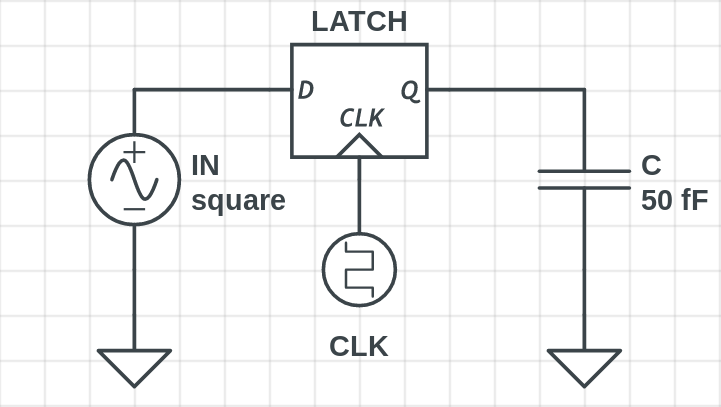
\includegraphics[scale=0.5]{images/schem_pretty.png}
\end{figure}

\chapter{Proposta}\label{proposta}
A proposta do relatório é construir e realizar a medição de métricas de implementações do \textbf{somador de 4 bits} na tecnologia CMOS C35B4 da \textit{Austria Microsystems}, utilizando valores de W\textsubscript{p} e de W\textsubscript{n} dessas respectivas portas conforme a Tabela \ref{tab:imp} e uma lógica de transistores de passagem.
Além disso, o circuito também deverá seguir às seguintes especificações:

%TODO: 
\begin{itemize}[noitemsep]
    \setlength{\itemindent}{1em}
    \item VDD = \SI{3.3}{\V};
    \item $1/{f_{clk}}$ = \SI{20}{\ns};
    \item Tclk\textsubscript{rise} = \SI{200}{\ps};
    \item Tclk\textsubscript{fall} = \SI{200}{\ps};
\end{itemize}

Criados o leiaute, é obrigatório tanto o teste individual utilizando as ferramentas \textit{DRC} e \textit{LVS} quanto a extração das capacitâncias parasitas da implementação.

\begin{table}[ht]
    \centering
    \caption{Dimensões da implementação.}
    \label{tab:imp}
    \begin{tabular}{l c c}
        \hline
        Implementação
        & W\textsubscript{p}
        & W\textsubscript{n} \\ \hline
        Latch tipo D & \SI{3.0}{\um}    & \SI{1.5}{\um}     \\ \hline
    \end{tabular}
\end{table}

\chapter{Análise}\label{analise}
Neste capítulo abordaremos a implementação da Latch tipo D e, no Capítulo \ref{resultados}, analisaremos os resultados e faremos algumas observações sobre o circuito simulado.

A Figura \ref{fig:latch} mostra o esquemático do circuito, que utiliza inversores \textit{tri-state} nesta escolha de implementação. Além disso, nessa versão uma entrada de relógio atuará como enable.
 
\begin{figure}[htbp]
    \centering
    \caption{Esquemático da Latch tipo D usando inversores \textit{tri-state}.}
    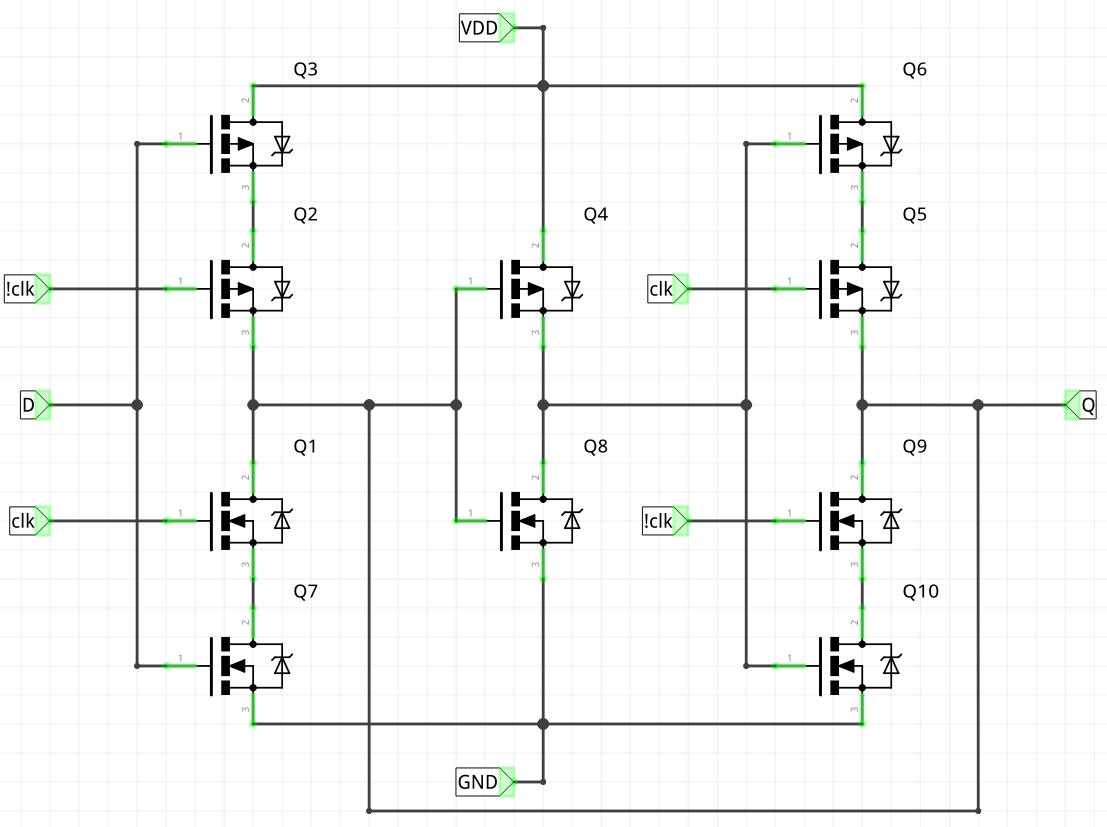
\includegraphics[scale=0.5]{images/schem_pretty_transistors.png}
    \label{fig:latch}
\end{figure}

\section{Latch tipo D}\label{nand}
A Latch tipo D, como vista anteriormente na Tabela \ref{tab:imp}, possuirá transistores PMOS e NMOS dimensionados respectivamente em \SI{3.0}{\um} e \SI{1.5}{\um}, e, assim como nas aula práticas anteriores, as células projetadas tem \SI{14}{\um} de altura num processo CMOS de substrato P\textsuperscript{-}.

A Figura \ref{fig:esquematico} mostra o esquemático da porta lógica na ferramenta \virtuoso, e a Figura \ref{fig:leiaute} mostra o seu respectivo leiaute. O leiaute foi feito manualmente sem utilizar as ferramentas de automação e de simplificação do processo de criação de leiaute do \virtuoso.

Como adicional, podemos observar na Figura \ref{fig:capacitancias} as capacitâncias extraidas do leiaute da Figura \ref{fig:leiaute}.

\begin{figure}[htbp]
    \centering
    \caption{Esquemático da Latch tipo D}
    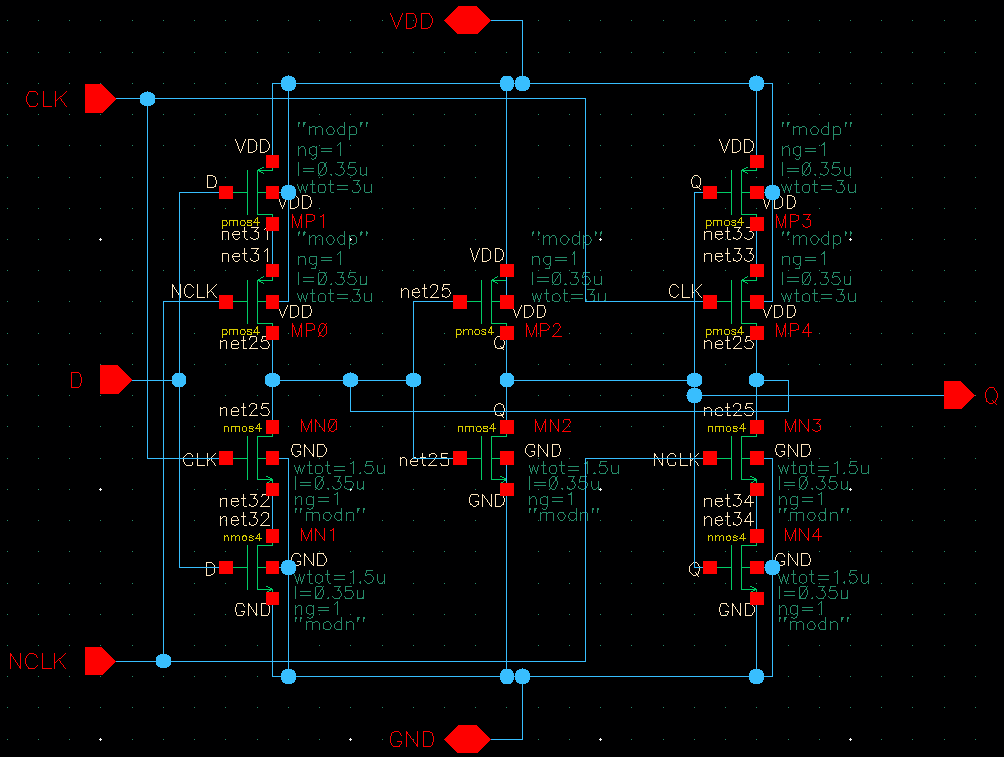
\includegraphics[scale=0.55]{images/schem_transistor.png}
    \label{fig:esquematico}
\end{figure}

\begin{figure}[htbp]
    \centering
    \caption{Leiaute da Latch tipo D}
    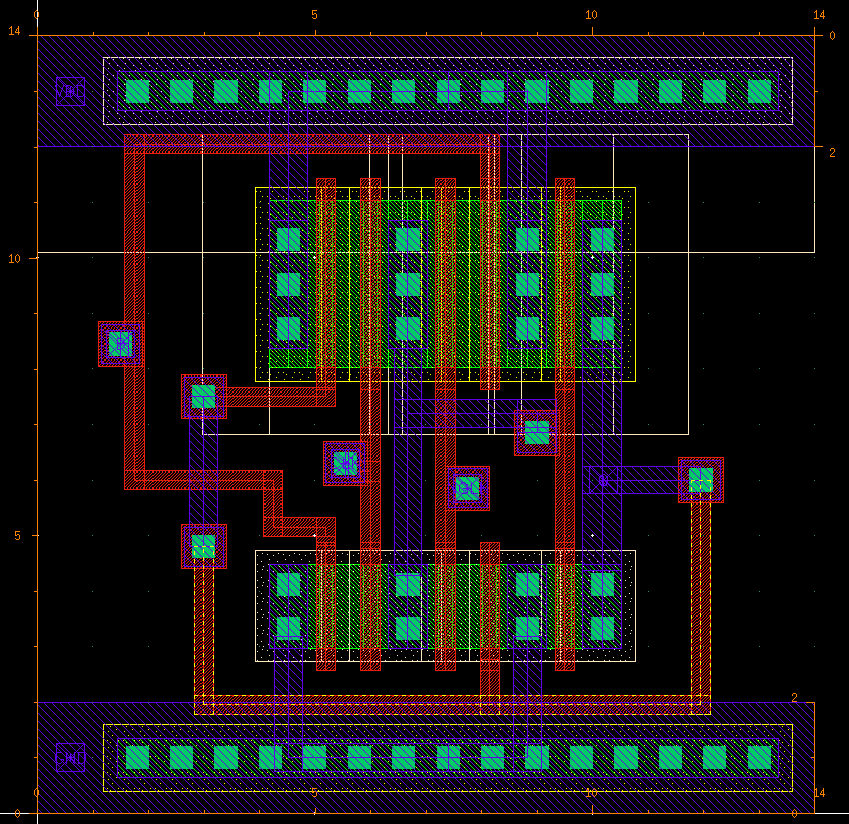
\includegraphics[scale=0.65]{images/lay.png}
    \label{fig:leiaute}
\end{figure}

\begin{figure}[htbp]
    \centering
    \caption{Capacitancias extraídas do leiaute da Latch tipo D}
    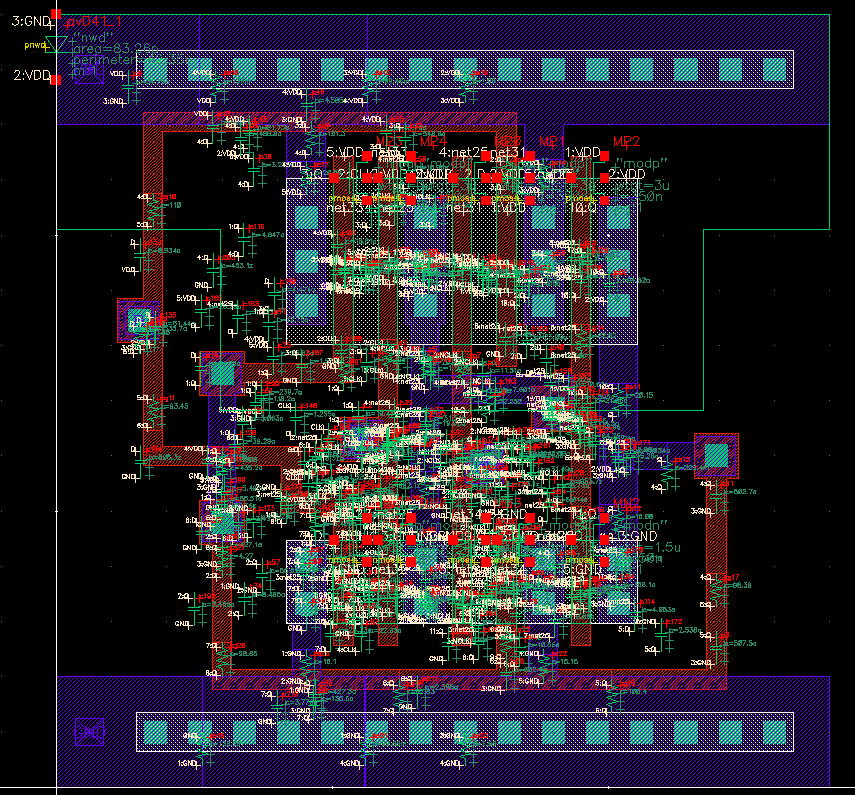
\includegraphics[scale=0.65]{images/cap.png}
    \label{fig:capacitancias}
\end{figure}

\FloatBarrier

Os resultados da análise transiente desse circuito estão no Capítulo \ref{resultados}.\

A Figura \ref{fig:trans} mostra o esquemático do circuito na ferramenta \virtuoso, e a Figura \ref{fig:wave} mostra o \textit{waveform} da simulação transiente do circuito.

\begin{figure}[htbp]
    \centering
    \caption{Esquemático da simulação transiente do circuito.}
    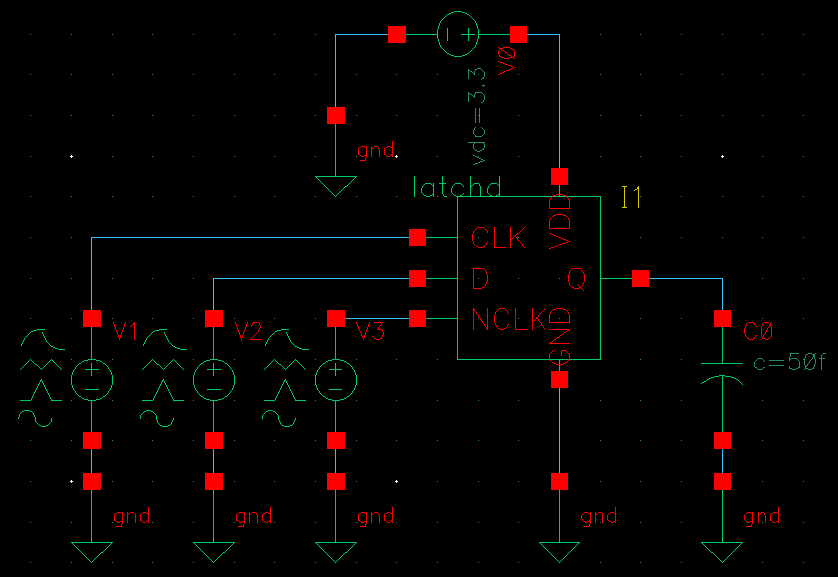
\includegraphics[scale=0.55]{images/schem.png}
    \label{fig:trans}
\end{figure}

\begin{figure}[htbp]
    \centering
    \caption{Waveforms da simulação transiente do circuito.}
    \subfloat[united]{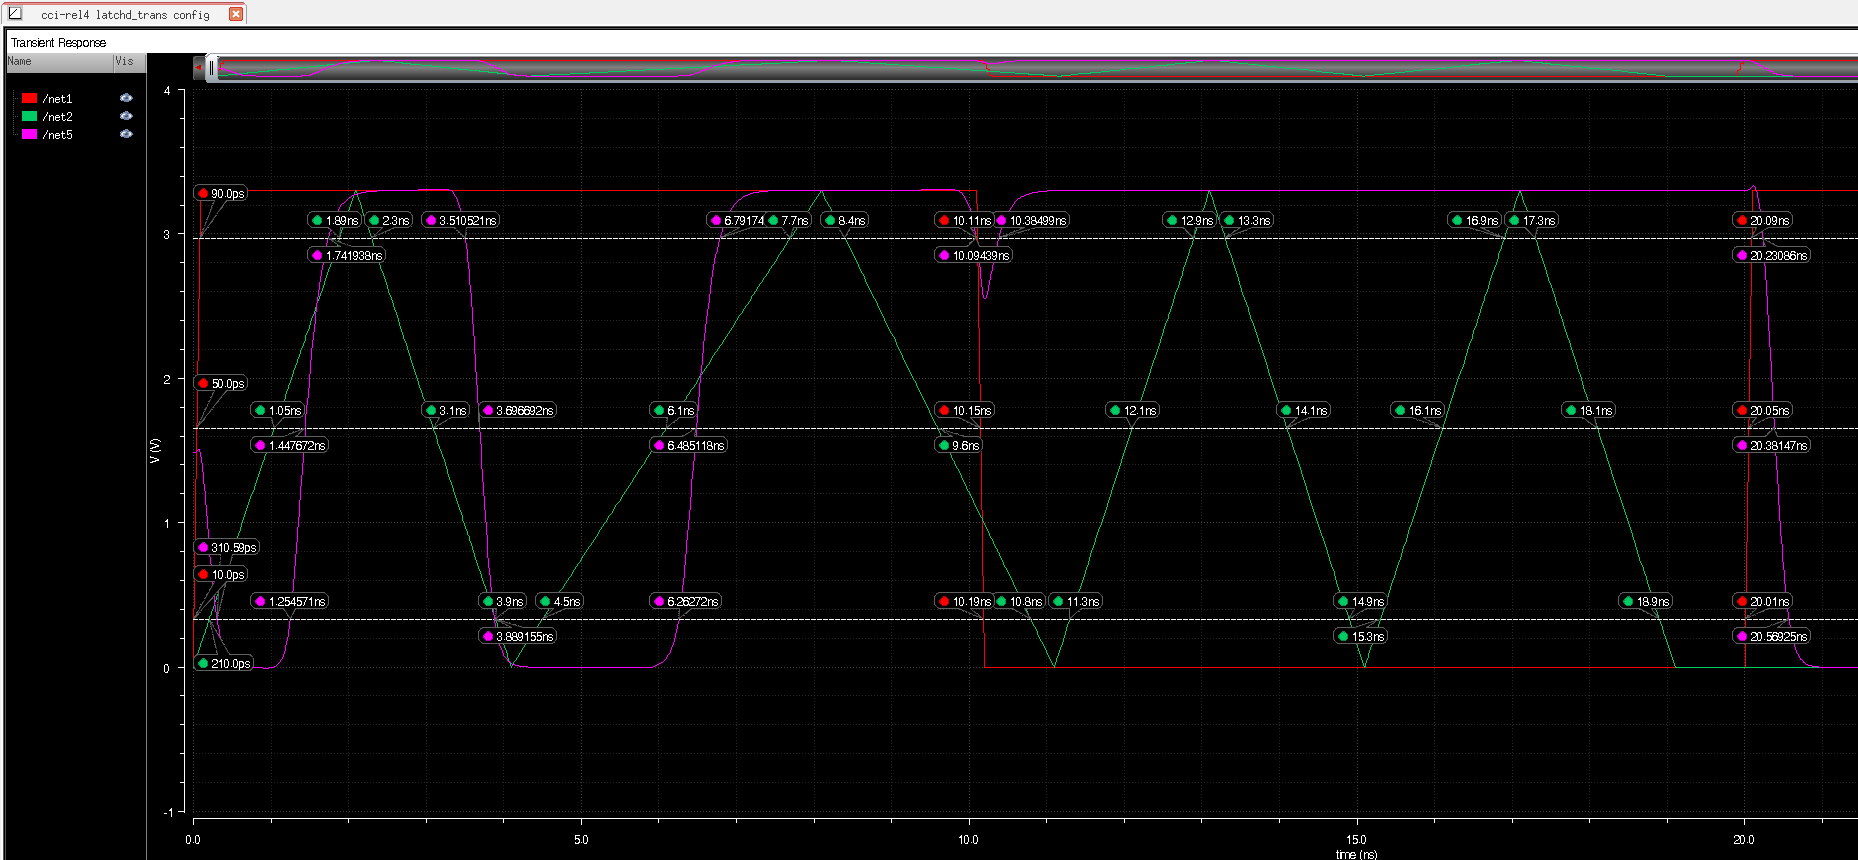
\includegraphics[scale=0.3]{images/wave_united.png}} \\
    \subfloat[separated]{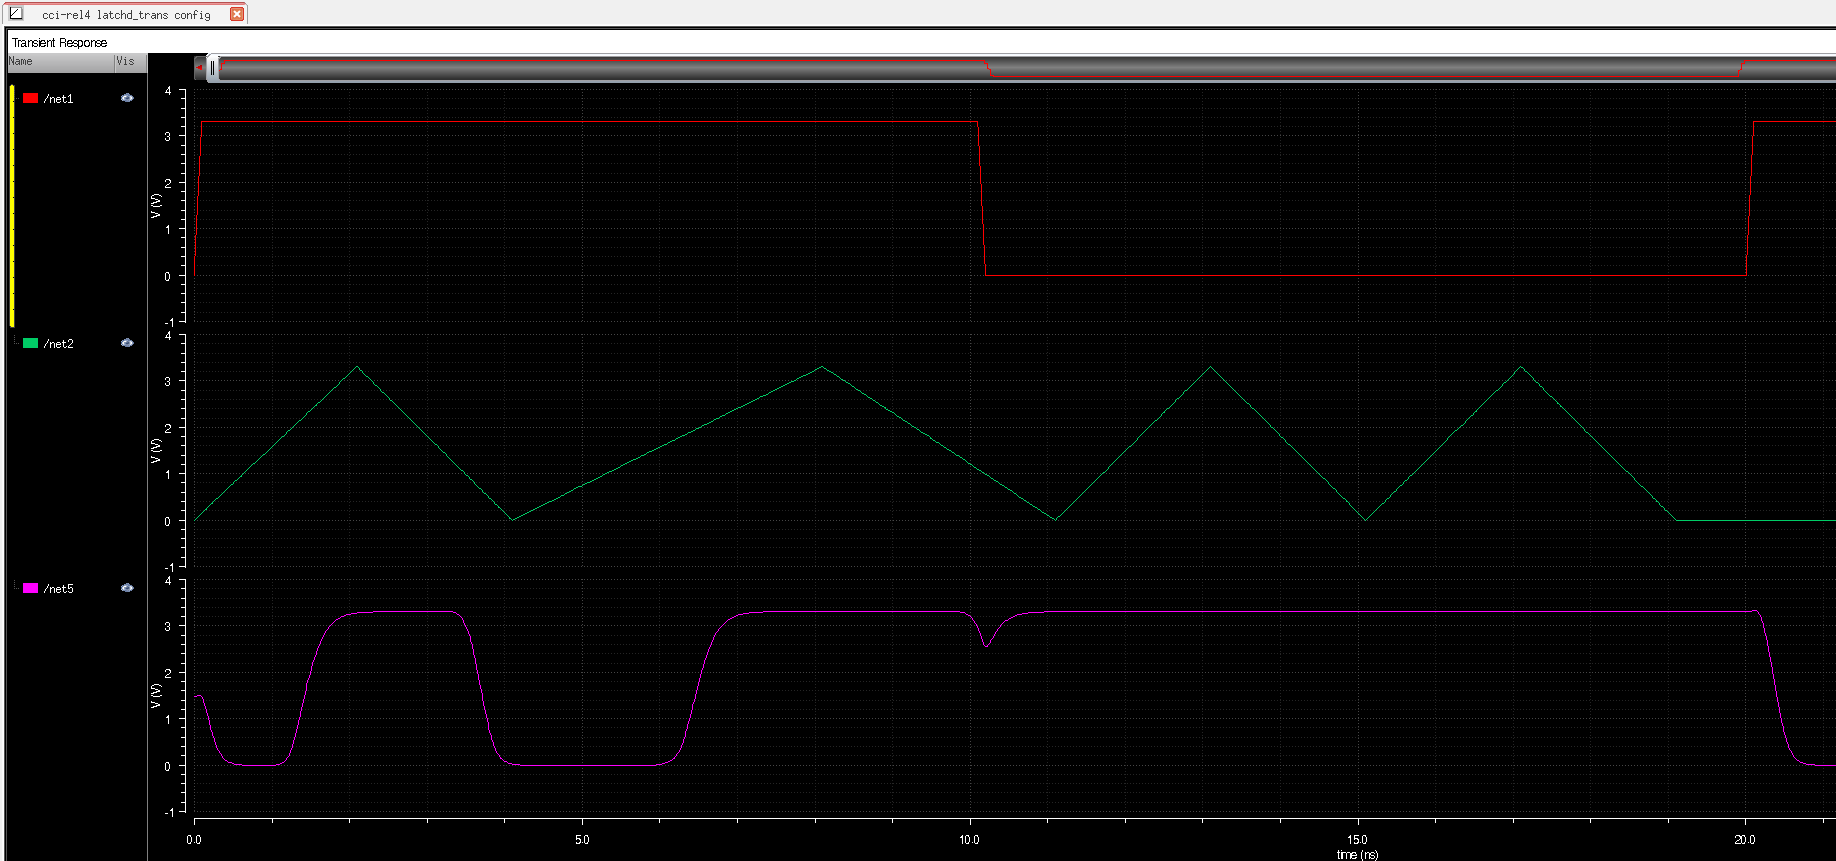
\includegraphics[scale=0.3]{images/wave_sep.png}}
    \label{fig:wave}
\end{figure}

\FloatBarrier

Eu utilizei um teste auxiliar para obter as métricas de tempo do circuito. A as Figuras \ref{fig:timing} mostram o resultado dessa simulação, que foi obtida variando a entrada D por uma curva quadrada de período 6ns.

\begin{figure}[htbp]
    \centering
    \caption{Waveforms da simulação de timings do circuito.}
    \subfloat[united]{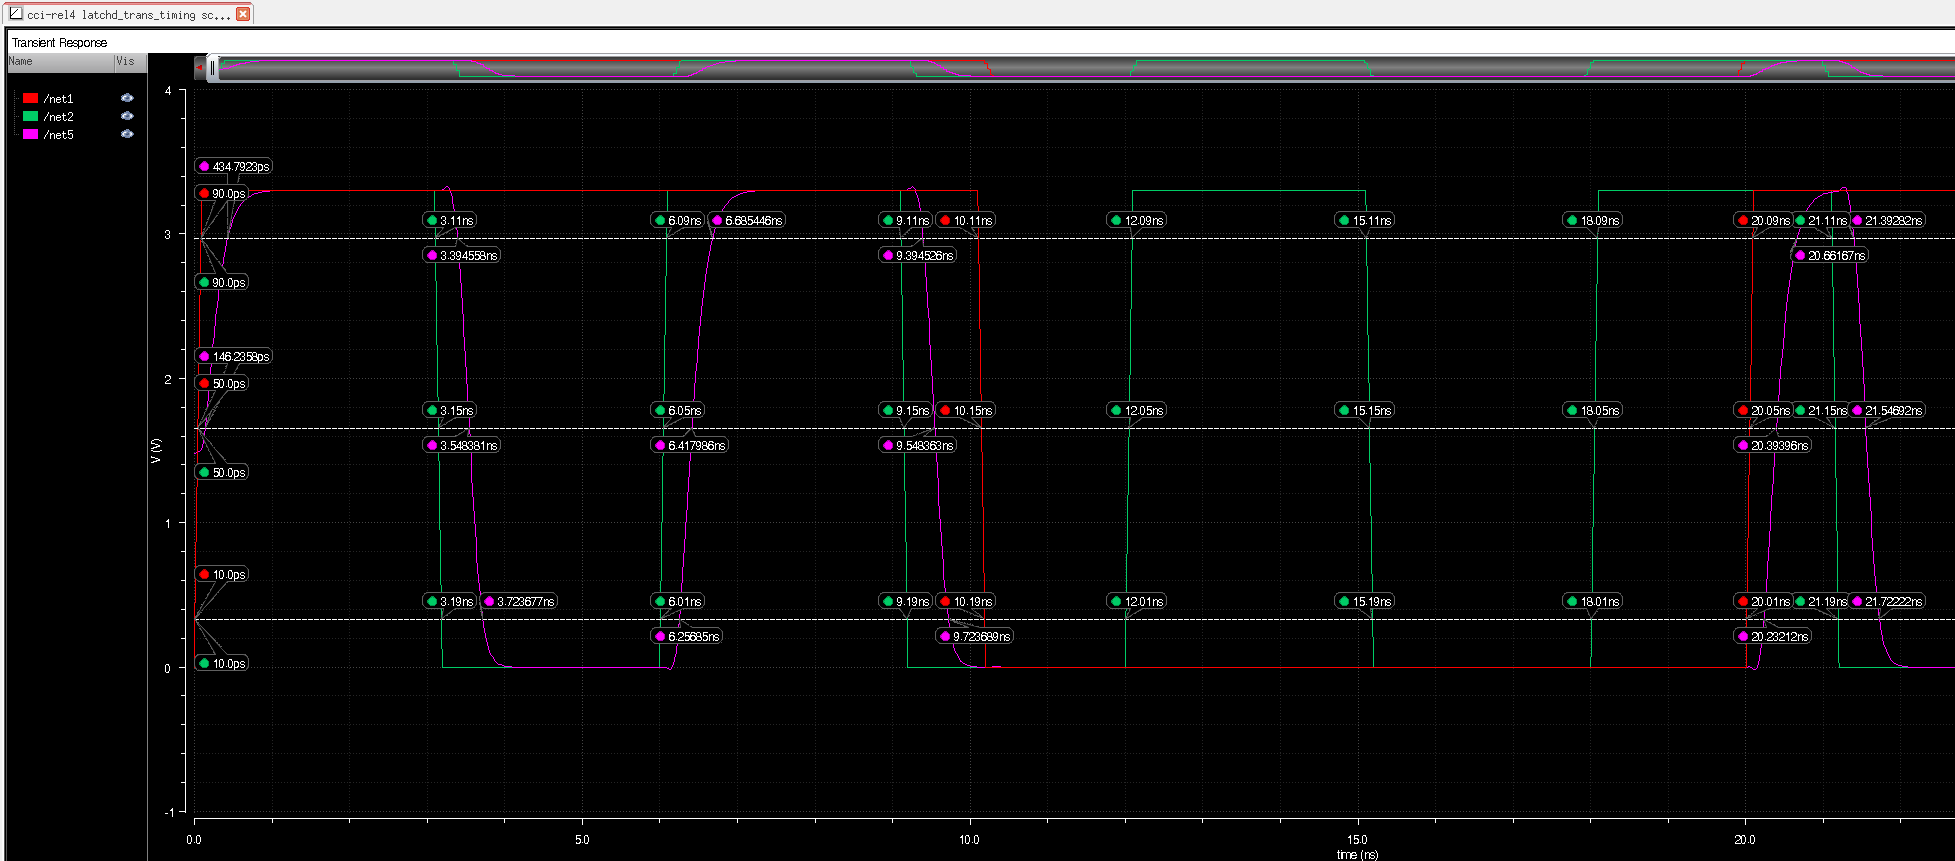
\includegraphics[scale=0.3]{images/timing_united.png}} \\
    \subfloat[separated]{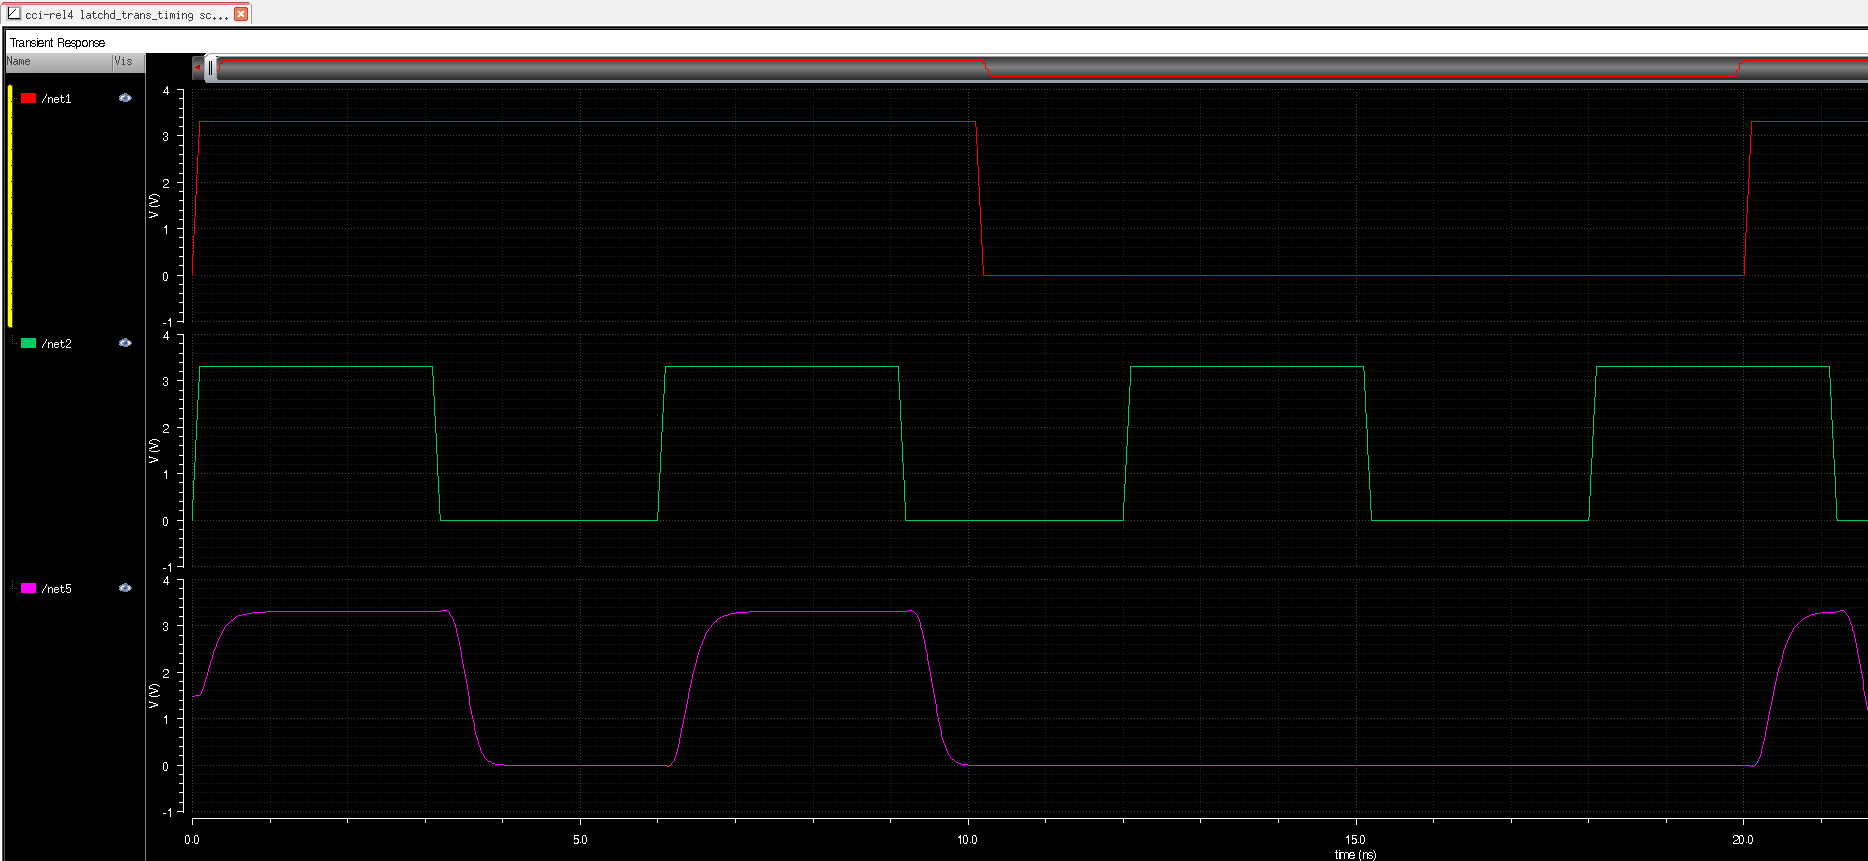
\includegraphics[scale=0.3]{images/timing_sep.png}}
    \label{fig:timing}
\end{figure}

\chapter{Resultados}\label{resultados}
Neste capítulo abordaremos os resultados obtidos nas simulações.

\section{Tabela}\label{tabela}
A Tabela \ref{tab:tempo} define os valores encontrados para as métricas temporais definidas no Capítulo \nameref{intro} para o circuito\footnote{Visto que é impossível uma combinação de entradas válidas que fazem o circuito variar de maneira LH ou HL, analisei as métricas \textit{Low-Low} e \textit{High-High} por meio da simulação adicional apresentada na Figura \ref{fig:timing}}, e a Tabela \ref{tab:potencia} define as métricas de energia para o mesmo dito circuito.

\begin{table}[ht]
    \centering
    \caption{Resultados temporais das simulações.}
    \small
    \label{tab:tempo}
    \sisetup{scientific-notation = true, round-mode = places, round-precision = 3}
    \begin{tabular}{l l l l l l}
        \hline
        Porta
        & Tp\textsubscript{LL}
        & Tp\textsubscript{HH}
        & Tp\textsubscript{médio}
        & T\textsubscript{LH}
        & T\textsubscript{HL} \\ \hline
        Latch tipo D
        & \SI{0.398381}{\ns} & \SI{0.367986}{\ns} & \SI{0.3831835}{\ns} & \SI{0.428596}{\ns}
        & \SI{0.329119}{\ns} \\
        \hline
    \end{tabular}
\end{table}

\begin{table}[ht]
    \centering
    \caption{Resultados de consumo de potência.}
    \small
    \label{tab:potencia}
    \sisetup{scientific-notation = true, round-mode = places, round-precision = 3}
    \begin{tabular}{l l l}
        \hline
        $\cdots$
        & P\textsubscript{média}
        & P\textsubscript{RMS} \\ \hline
        Latch tipo D
        & \SI{127.2e-6}{\W}  & \SI{319.4e-6}{\W} \\
        \hline
    \end{tabular}
\end{table}

%%%%%%%%%%%%%%%%%%%%%%%%%%%%%%%%%%%%%%%%%%%%%%%%%%%%%%%%%%%%%%

%\bibliographystyle{abntex2-alf}
%\bibliography{biblio} 

\end{document}
